\chapter{Execução à nível de Time}

  Esse capítulo apresenta as atividades e resultados obtidos na execução do processo a nível de Time.
  
  \begin{figure}[!htbp]
    \centering
    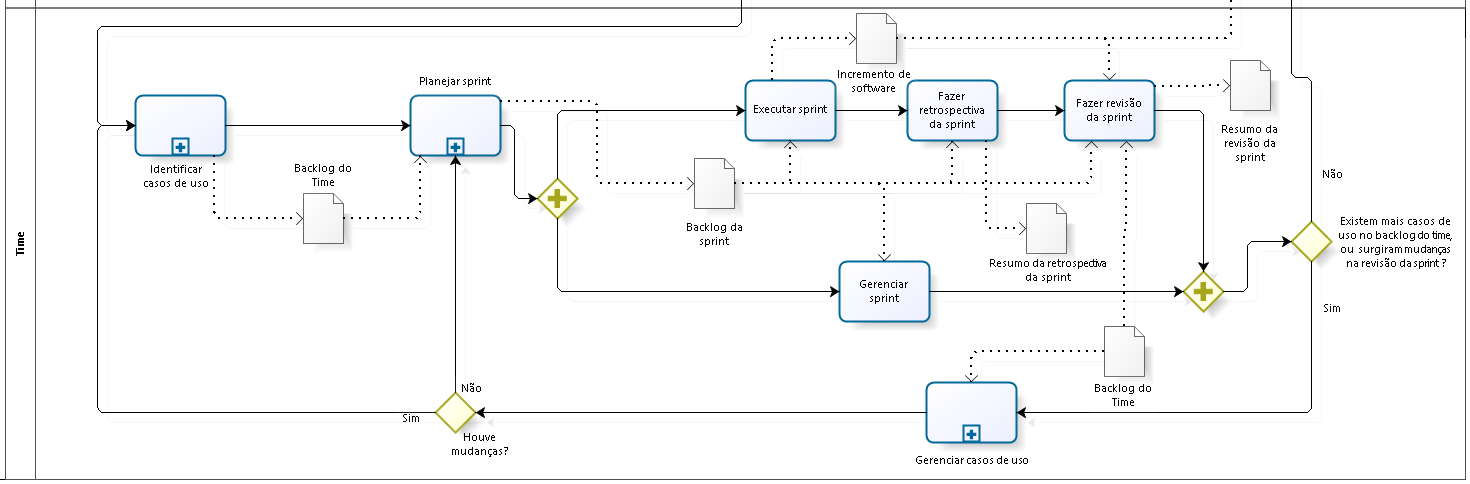
\includegraphics[scale=0.33]{figuras/processo_time}
    \caption[Processo - Nível de Time]{Processo - Nível de Time.}
    \label{processo_time}
  \end{figure}
  
  \section{Reuniões realizadas}
  
  
  \section{Especificação dos Casos de Uso}
 
  Foram especificados os casos de uso:
  
  \begin{itemize}
    \item Cadastrar missão;
    \item Alterar missão;
    \item Consultar missão;
    \item Gerenciar vínculo entre viaturas e missões
    \item Cadastrar motorista;
    \item Alterar motorista;
    \item Consultar motorista;
    \item Inativar motorista;
    \item Gerenciar vínculo entre motoristas e viaturas;
    \item Cadastrar viatura;
    \item Alterar viatura;
    \item Consultar viatura;
    \item Inativar viatura.
  \end{itemize}

  
  Os mesmos se encontram no Apêndice \ref{Especificacao}
  
  \section{Considerações finais a nível de Time}
    
    Esta seção apresenta um resumo dos itens mais importantes produzidos a nível de Time.
    
    \subsection{Casos de uso identificados} 
      
      O \textit{Backlog} do Time ficou composto pelos seguintes casos de uso:
      
      \subsubsection{F1UC1 - Cadastrar missão}
Este caso de uso permite ao Sargento de uma unidade do CBM-DF cadastrar dados de uma missão no sistema de gestão de viaturas para
manter os registros no sistema.

  \subsubsection{F1UC2 - Alterar missão}
Este caso de uso permite ao Sargento de uma unidade do CBM-DF alterar dados de uma missão no sistema de gestão de viaturas
para manter o registro no sistema.

  \subsubsection{F1UC3 - Consultar missão}
Este caso de uso permite ao Consultor operacional do CBM-DF consultar dados de missões no sistema de gestão de viaturas para
manter o registro no sistema.

  \subsubsection{F1UC4 - Gerenciar vínculo entre viaturas e missão}
Este caso de uso permite ao Sargento de uma unidade do CBM-DF associar uma viatura a missão no sistema de gestão de viaturas 
para manter o registro no sistema.

  \subsubsection{F1UC5 - Gerar relatório da missão}
Este caso de uso permite a um funcionário da gestão administrativa das unidades ou do Gestor Operacional gerar relatórios de
missões realizadas para verificar os dados existentes.

  \subsubsection{F2UC1 - Adicionar abastecimento}
Este caso de uso permite a adição de dados de abastecimento das viaturas das unidades do CBM-DF para manter o registro no sistema.

  \subsubsection{F2UC2 - Alterar abastecimento}
Este caso de uso permite a alteração de dados de abastecimento das viaturas das unidades do CBM-DF para manter o registro no sistema.

  \subsubsection{F2UC3 - Consultar abastecimento}
Este caso de uso permite a consulta dos dados de abastecimento das viaturas das unidades do CBM-DF para verificar os registros
do sistema.

  \subsubsection{F2UC4 - Inserir recibo do abastecimento}
Este caso de uso permite a inserção do recibo de abastecimento nos dados do abastecimento, quando este for cadastrado no 
sistema de gerenciamento de viaturas do CBM-DF para manter o registro no sistema.

  \subsubsection{F2UC5 - Gerar relatório do consumo de combustível}
Este caso de uso permite a um funcionário da gestão administrativa das unidades ou o Gestor Operacional gerar relatórios de
consumo de combustível por tipo de combustível, postos, motoristas, tipos de viaturas para verificar os dados existentes. 

  \subsubsection{F3UC1 - Consultar viaturas disponíveis nas unidades}
Este caso de uso permite a um Gestor Operacional consultar viaturas disponíveis em uma unidade do CBM-DF para verificar os 
dados existentes no sistema.

  \subsubsection{F3UC2 - Visualizar unidades no mapa}
Este caso de uso permite a um Gestor Operacional consultar unidades do CBM-DF no mapa para verificar os dados existentes no sistema.

  \subsubsection{F4UC1 - Criar escala}
Este caso de uso permite ao funcionário da gestão administrativa das unidades adicionar uma escala no sistema de
gerenciamento de viaturas do CBM-DF para manter o registro no sistema.

  \subsubsection{F4UC2 - Alterar escala}
Este caso de uso permite ao funcionário da gestão administrativa das unidades alterar uma escala no sistema de
gerenciamento de viaturas do CBM-DF para manter o registro no sistema.

  \subsubsection{F4UC3 - Consultar escala}
Este caso de uso permite ao funcionário da gestão administrativa das unidades consultar uma escala no sistema 
de gerenciamento de viaturas do CBM-DF para visualizar os registros do sistema.

  \subsubsection{F4UC4 - Excluir escala}
Este caso de uso permite ao funcionário da gestão administrativa das unidades  excluir uma escala no sistema 
de gerenciamento de viaturas do CBM-DF para deletar o registro do sistema.

  \subsubsection{F4UC5 - Cadastrar motorista}
Este caso de uso permite que o Gestor Operacional cadastre um motorista na corporação do CBM-DF para manter o registro no sistema.

  \subsubsection{F4UC6 - Consultar motorista}
Este caso de uso permite que o Gestor Operacional consulte um motorista na corporação do CBM-DF para verificar o registro no sistema.

  \subsubsection{F4UC7 - Alterar motorista}
Este caso de uso permite que o Gestor Operacional altere um motorista na corporação do CBM-DF para manter o registro no sistema.

  \subsubsection{F4UC8 - Inativar motorista}
Este caso de uso permite que o Gestor Operacional inative um motorista na corporação do CBM-DF para desativar o registro no sistema.

  \subsubsection{F4UC9 - Gerenciar vínculo entre motoristas e viaturas}
Este caso de uso permite a um Sargento vincular um motorista à uma viatura ou desvincular um motorista de uma viatura da unidade
para manter o registro no sistema.

  \subsubsection{F4UC10 - Gerar relatórios sobre dados dos motoristas}
Este caso de uso permite a um funcionário da gestão administrativa das unidades ou d]o Gestor Operacional gerar relatórios de 
motoristas por tipo de habilitação, tempo de vencimento de habilitação, nome, cursos completados e status para visualizar
o registro do sistema.

  \subsubsection{F4UC11 - Alocar motorista à unidade}
Este caso de uso permite que o Gestor Operacional designe um motorista a uma unidade do CBM-DF para manter o registro no sistema.

  \subsubsection{F5UC1 - Cadastrar viaturas}
Este caso de uso permite que o Gestor Operacional adicione viaturas ao sistema de gerenciamento de viaturas do CBM-DF 
para manter o registro no sistema.

  \subsubsection{F5UC2 - Consultar viaturas}
Este caso de uso permite a consulta de viaturas no sistema de gerenciamento de viaturas do CBM-DF para manter o registro no sistema.

  \subsubsection{F5UC3 - Alterar dados das viaturas}
Este caso de uso permite que o Gestor Operacional altere dados de viaturas no sistema de gerenciamento de viaturas do 
CBM-DF para manter o registro no sistema.

  \subsubsection{F5UC4 - Inativar viaturas}
Este caso de uso permite que o Gestor Operacional desative viaturas no sistema de gerenciamento de viaturas do CBM-DF para 
manter o registro no sistema.

  \subsubsection{F5UC5 - Alocar viatura em uma unidade}
Este caso de uso permite que o Gestor Operacional atribua uma unidade de operação específica a uma viatura para manter o 
registro no sistema.

  \subsubsection{F5UC6 - Estabelecer custo do combustível}
Este caso de uso permite que o Gestor Operacional estabeleça e modifique o custo do combustível para abastecimento
das viaturas do CBM-DF para manter o registro no sistema.

  \subsubsection{F5UC7 - Gerar relatórios referentes a dados das viaturas}
Este caso de uso permite a um funcionário da gestão administrativa das unidades gerar relatórios de viaturas das
unidades ou o Gestor Operacional gerar relatórios de todas as viaturas de todas as unidades por tipo de viaturas,
estado da viatura e unidades de alocação para visualizar o registro do sistema.
